\documentclass[border=2mm,tikz,preview]{standalone}
               
\usetikzlibrary{positioning,chains}

\begin{document}

% Tikz commands based on https://tex.stackexchange.com/a/263761

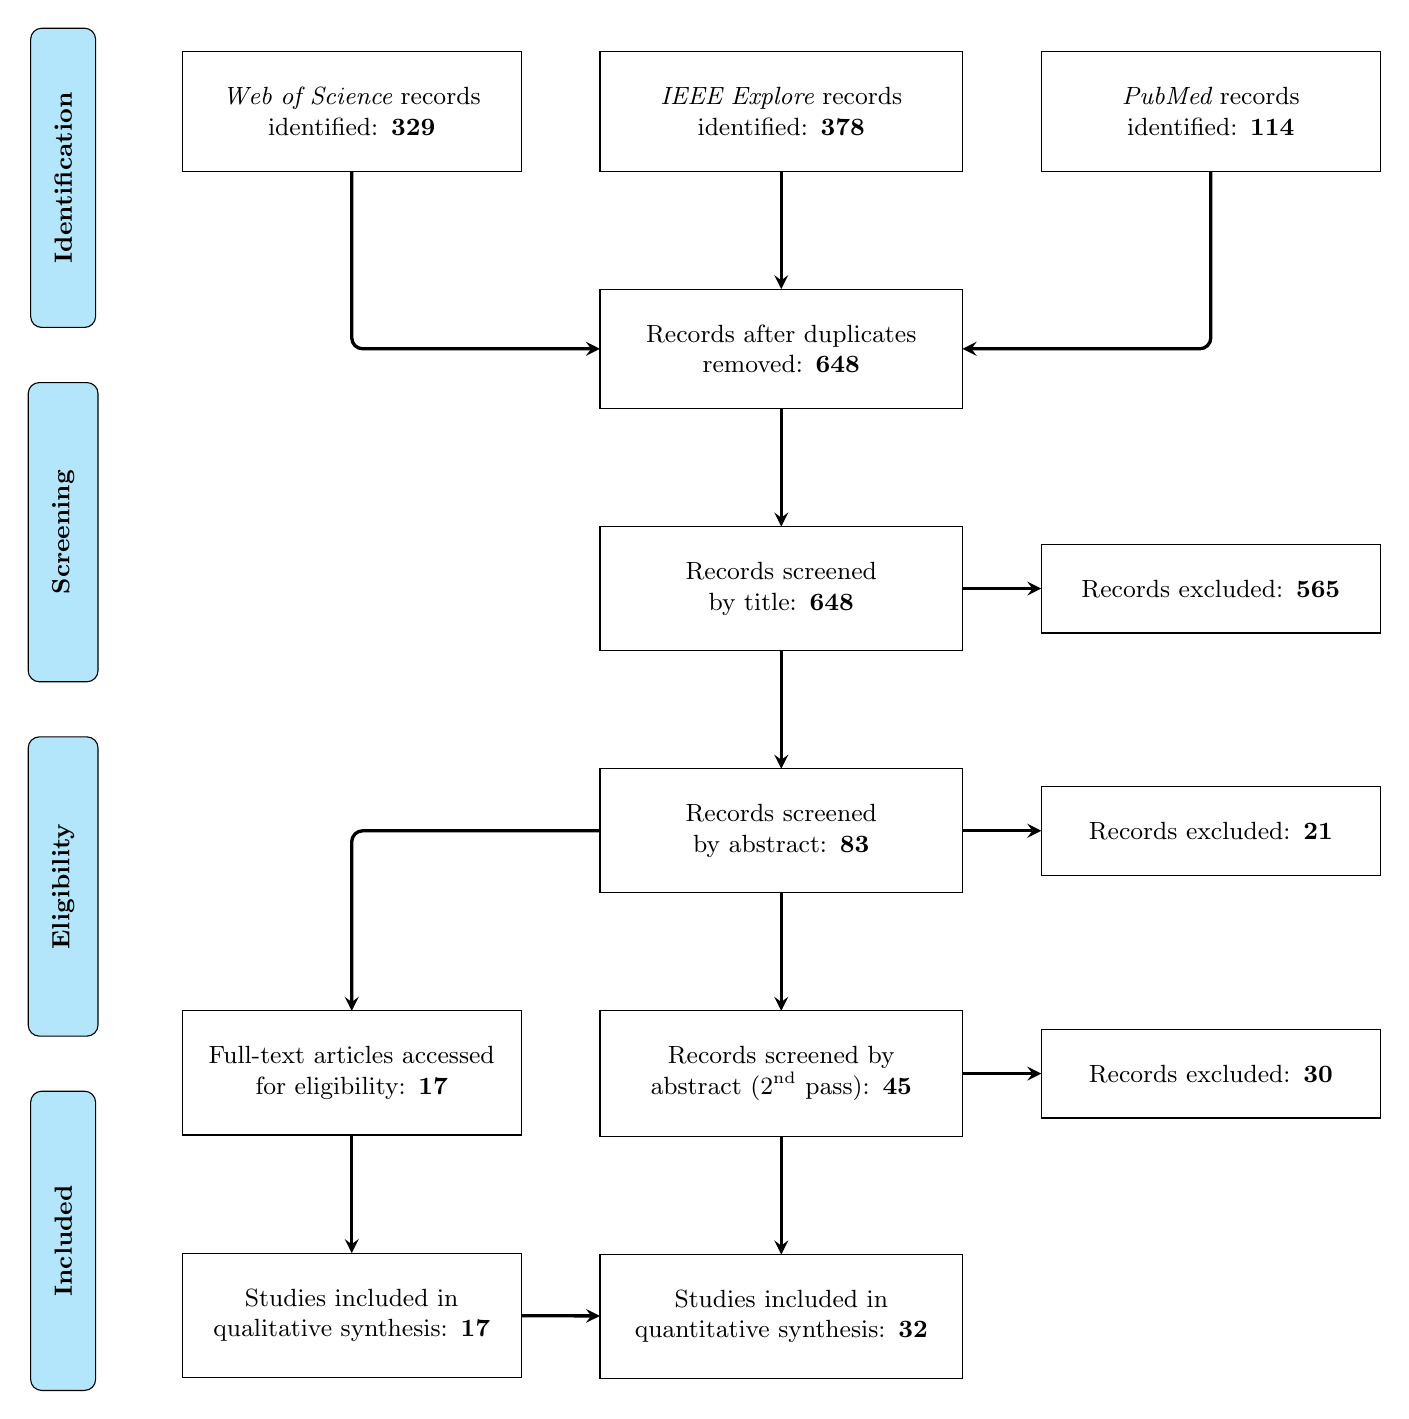
\begin{tikzpicture}[
	node distance=15mm and 10mm,
	start chain=going below,
	mynode/.style = {
		draw, rectangle, align=center, text width=4cm,
		font=\small, inner ysep=3ex, inner xsep=2ex, 
		outer sep=0pt, on chain},
	smallnode/.style = {
		mynode, text width=3.7cm
	},
	mylabel/.style = {
		draw, rectangle, align=center, rounded corners, 
		font=\small\bfseries, inner sep=2ex, outer sep=0pt,
		fill=cyan!30, minimum height=38mm,
		on chain},
	every join/.style = arrow,
	arrow/.style = {very thick, -stealth, rounded corners}
]
\coordinate (tc);

%\node[above=of tc,font=\bfseries] {PRISMA 2009 Flow Diagram};

\node (n1a) [smallnode, left=of tc]    {{\it Web of Science} records identified: {\bf 329}};
\node (n1b) [mynode,right=of n1a]    {{\it IEEE Explore} records\\ identified: {\bf 378 }};
\node (n1c) [smallnode,right=of n1b]    {{\it PubMed} records\\ identified: {\bf 114 }};

\node (n2)  [mynode, below=of n1b]   {Records after duplicates\\
                                     removed: {\bf 648}};
\node (n3a)  [mynode,join]   {Records screened\\ by title: {\bf 648}};
\node (n3b)  [mynode,join]   {Records screened\\ by abstract: {\bf 83}};
\node (n3c)  [mynode,join]   {Records screened by abstract (2\textsuperscript{nd} pass): {\bf 45}};
\node (n4)  [smallnode] at (n1a |- n3b.south)  {Full-text articles accessed 
                             for eligibility: {\bf 17}};
\node (n6)  [smallnode,join]   {Studies included in
                             qualitative synthesis: {\bf 17}};
\node (n5)  [mynode, below=of n3c]   {Studies included in
                             quantitative synthesis: {\bf 32}};

\node (n3ar) [smallnode,right=of n3a]    {Records excluded: {\bf 565}};
\node (n3br) [smallnode,right=of n3b]    {Records excluded: {\bf 21}};
\node (n3cr) [smallnode,right=of n3c]    {Records excluded: {\bf 30}};
                                    
\draw[arrow] (n1a.south) coordinate (b) -- (b |- n2.west) -- (n2.west);
\draw[arrow] (n1b.south) coordinate (b) -- (b |- n2.north);
\draw[arrow] (n1c.south) coordinate (b) -- (b |- n2.east) -- (n2.east);
\draw[arrow] (n3b.west) -- (n4 |- n3b) -- (n4.north);
\draw[arrow] (n3a) -- (n3ar);
\draw[arrow] (n3b) -- (n3br);
\draw[arrow] (n3c) -- (n3cr);
\draw[arrow] (n3c) -- (n5);
\draw[arrow] (n6) -- (n5);

	\begin{scope}[node distance=7mm]
		\node[mylabel,below left=-3mm and 11mm of n1a.north west]
						{\rotatebox{90}{Identification}};
		\node[mylabel]  {\rotatebox{90}{Screening}};
		\node[mylabel]  {\rotatebox{90}{Eligibility}};
		\node[mylabel]  {\rotatebox{90}{Included}};
	\end{scope}
\end{tikzpicture}

\end{document}
